\documentclass{standalone}
\usepackage{tikz}
\begin{document}
	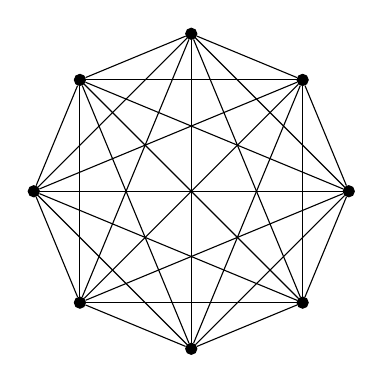
\begin{tikzpicture} [transform shape]
		\foreach \x in {1,...,8}{%
    		\pgfmathparse{(\x-1)*45+floor(\x/9)*22.5}
	    	\node[draw,circle,inner sep=0.05cm, fill] (N-\x) at (\pgfmathresult:2.0cm) {};
  	} 
	  \foreach \x [count=\xi from 1] in {2,...,8}{%
    	\foreach \y in {\x,...,8}{%
    	\path (N-\xi) edge (N-\y);
  	}
	}
	\end{tikzpicture}
\end{document}